\documentclass[palatino,nosec]{Docencia}


\title{Examen modelo con solución (4ºA)}

\author{Departamento de Matemáticas}
\date{17/18}


% Paquetes adicionales

\usepackage[author={Víctor de Juan, 2017}]{pdfcomment}

\usepackage{pgf,tikz}
\usetikzlibrary{arrows}


\definecolor{qqttcc}{rgb}{0,0.2,0.8}
\definecolor{qqqqff}{rgb}{0,0,1}
\definecolor{cccccc}{rgb}{0.8,0.8,0.8}


\makeatletter
\newcommand{\annotate}[2][]{%
\pdfstringdef\x@title{#1}%
\edef\r{\string\r}%
\pdfstringdef\x@contents{#2}%
\pdfannot
width 2\baselineskip
height 2\baselineskip
depth 0pt
{
/Subtype /Text
/T (\x@title)
/Contents (\x@contents)
}%
}
\makeatother



\usepackage{eso-pic}
\newcommand\BackgroundPic{%
\put(0,0){%
\parbox[b][\paperheight]{\paperwidth}{%
\vfill
\centering

\includegraphics[width=\paperwidth,height=\paperheight,%
keepaspectratio]{../../../../BWLogo.jpeg}%
\vfill
}}}





\begin{abstract}
Solución del primer parcial de la segunda evaluación.

\nota{Estos ejemplos no están exentos de erratas. En caso de descubrir alguna, por favor, comunicarlas.}
\end{abstract}

% --------------------
\newcommand{\cimplies}{\text{\hl{$\implies$}}}

\begin{document}
\pagestyle{plain}
\maketitle

\AddToShipoutPicture{\BackgroundPic}

\begin{problem} (1.5 puntos)

Calcula las siguientes razones trigonométricas:

\ppart $\cos(-225º)$
\ppart $\sen(1170º)$
\ppart $\cos(6π\;rad)$
\solution

\spart $\cos(-225º) = \cos(225º) = -\cos(225-180) = -\cos(45) = \rfrac{\sqrt{2}}{2}$

\spart $\sen(1170º) = \sen(1170-720) = \sen(330) = -\sen(360-330) = -\sen(30) = -\rfrac{1}{2}$

\spart $\cos(6π\;rad) = \sen(6π - 3·2π) = \sen(0) = 1$

\end{problem}

\begin{problem}(1.5 puntos)
Sabiendo que $\cosec(α) = +\sqrt{10}$ y que $90º<α<180º$, halla las demás razones trigonométricas. Ten en cuenta el cuadrante para el signo de cada razón trigonométrica. Deja los resultados en forma de fracción.

\solution

\[
	\left.
	\begin{array}{c}
		\cosec(α) = +\sqrt{10}\\
		\cosec(α) = \frac{1}{\sen(α)}
	\end{array}
	\right\} \to \sen(α) = \frac{1}{\cosec(α)} = \frac{1}{\sqrt{10}} = \frac{\sqrt{10}}{10}
\]

\[
	\left.
	\begin{array}{c}
		\cosec(α) = +\sqrt{10}\\
		\cosec^2(α) = 1 + \cotg^2(α)
	\end{array}
	\right\} \to 10 = 1+\cotg^2(α) \implies \cotg(α) = \pm\sqrt{9}
\]

Como $α$ está en el segundo cuadrante, la tangente y la cotangente son negativas, por lo que elegiremos la raíz negativa.

$\cotg(α) = -3$

\[
	\left.
	\begin{array}{c}
		\cotg(α) = -3\\
		\cotg(α) = \frac{1}{\tg(α)}
	\end{array}
	\right\} \to \tg(α) = \frac{1}{\cotg(α)} = \frac{1}{-3} = -\frac{1}{3}
\]

\[
	\left.
	\begin{array}{c}
		\tg(α) = -\frac{1}{3}\\
		\tg(α) = \frac{\sen(α)}{\cos(α)}
	\end{array}
	\right\} \to \cos(α) = \frac{\sen(α)}{\tg(α)} = \frac{\rfrac{\sqrt{10}}{10}}{\rfrac{-1}{3}} \implies \cos(α) = \frac{-3\sqrt{10}}{10}
\]
\end{problem}


\begin{problem}
Resuelve el siguiente triángulo:


\solution
\begin{figure}[h]
\centering
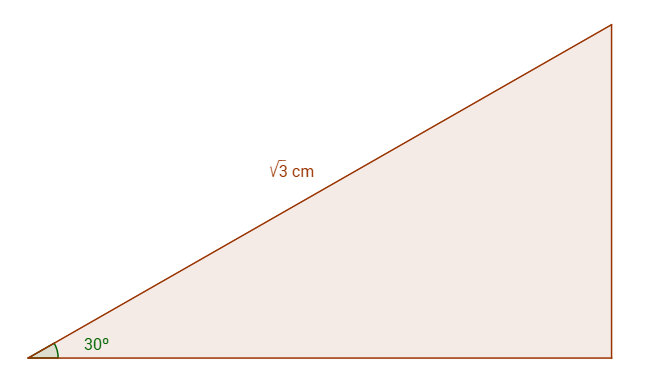
\includegraphics[scale=0.3]{Triang}
\end{figure}

\[
	\sen(30) = \frac{h}{\sqrt{3}} \implies h = \sen(30)\sqrt{3} = \frac{\sqrt{3}}{2}
\]
\end{problem}


\begin{problem}
Para financiar el viaje de fin de curso, los alumnos van a confeccionar y vender
adornos de 2 tipos. Cuentan con 1200 bolas blancas y 28 metros de hilo. Para hacer muñecos
de nieve necesitan 15 bolas blancas y 20 cm de hilo. Para hacer estrellas necesitan 40 cm de
hilo y 10 bolas blancas. Representa gráficamente cuántos adornos de cada tipo podrán
fabricar.
\solution

\begin{table}[hbtp]
\centering
\begin{tabular}{ccc}
&Bolas & Hilo\\
Muñecos & 15 & 20cm\\
Estrellas & 10 & 40cm
\end{tabular}
\end{table}

Como la limitación está en la cantidad de hilo y de bolas blancas, las incóngnitas serán la cantidad muñecos $x$ y las estrellas $y$.

\[
\left\{
	\begin{array}{c}
		15x + 10y ≤ 1200\\
		20x + 40y ≤ 2800
	\end{array}
\right\}
\]

\begin{figure}[h]
\centering
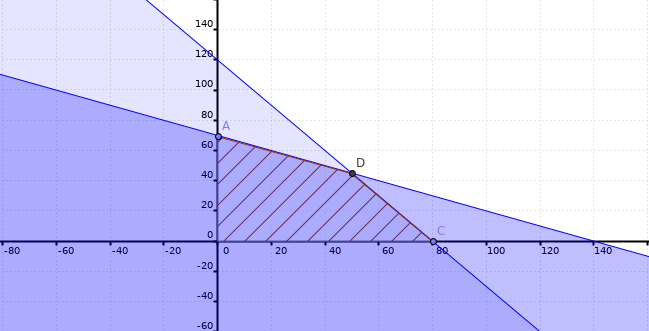
\includegraphics[scale=0.7]{Problema}
\caption{Solución gráfica}
\label{prob5}
\end{figure}

\end{problem}

\begin{problem}

Resuelve la siguiente ecuación trigonométrica: $\sec x = \sqrt{2}$

\solution

$\sec x = \rfrac{1}{\cos x}$. Buscamos cuadrantes en los que el coseno sea positivo, es decir $I$ y $IV$.

Por otro lado:

\[
	\sec x = \sqrt{2} \dimplies \frac{1}{\cos(x)} = \sqrt{2} \dimplies \cos(x) = \frac{1}{\sqrt{2}} = \frac{\sqrt{2}}{2} 
\]

Los ángulos buscados son $45º$ y, pasando al cuarto cuadrante: $360-45 = 315º$

\[
	x_1 = 45º + 360ºk\;\;,\;\; ∀k∈ℤ
\]
\[
	x_2 = 315º + 360ºk\;\;,\;\; ∀k∈ℤ
\]

\end{problem}

\begin{problem}
Resuelve la siguiente inecuación:

\[
	\frac{x^2-4x+8}{x+2}≤1
\]

\solution

\[
	\frac{x^2-4x+8}{x+2} - 1 ≤ 0 \dimplies \frac{x^2-4x+8-x-2}{x+2} ≤ 0 \dimplies \frac{x^2-5x+6}{x+2}≤0
\]
\[
	\frac{(x-2)(x-3)}{x+2}≤0
\]
Construimos la tabla
\[
\begin{array}{ccccc}
&(-\infty,-2.0)&(-2.0,2.0)&(2.0,3.0)&(3.0,\infty)\\
(x-2)&-&-&+&+\\
(x-3)&-&-&-&+\\
(x+2)&-&+&+&+\\
\frac{(x-2)(x-3)}{x+2} & - & + & - & + \\
\end{array}
\]

\textbf{Solución:} $(-2.0,2.0] ∪ [3.0,\infty)$

\end{problem}

\end{document}
